\documentclass{article}
\usepackage[utf8]{inputenc}
\usepackage{amsmath,amssymb, amsfonts}

\title{Método multiescala aplicado à problemas de geomecânica}
\author{Mateus Figueiredo}
\date{August 2018}

\usepackage{natbib}
\usepackage{graphicx}

\begin{document}

\maketitle

\section{Introdução}




\section{Discretização e Elementos Finitos \label{ch:discretizacao}}


\section{Método Multiescala}

\subsection{Construção do Operador Grosso}

Nessa seção é apresentado a construção de um operador multiescala para aplicação em um problema de elementos finitos. A construção desse tipo de operador tem diversas aplicações para a solução dos sistemas lineares apresentados advindos da discretização de equações diferenciais. Ele consiste basicamente em construir um operador grosso através do cálculo de funções de base em um grid gerado pelo acoplamento de elementos do grid fino. Pode ser utilizado como pré-condicionador \cite{casteletto}, como solver multinível semelhante aos solver multigrid ou ainda como aproximação para a solução original do problema. Os métodos multiescala tem sido aplicados com sucesso para problemas elípticos que é o caso do problema da elasticidade linear aqui apresentado. As vantagens do método apresentadas em \cite{thomashou} são que a funções de base multiescala tentam se adaptar as propriedades locais do operador de forma que o operador grosso as conserve, e também podem ser construídas através da solução de problemas independentes e, portanto, em paralelo.

O primeiro passo para a construção do operador multiescala é gerar um novo grid com menos elementos que o grid original do problema (grid fino) que ainda representa o mesmo domínio $\Omega$. Esse grid novo será chamado de grid grosso e as variáveis relacionadas com ele serão assinadas com o sobre-escrito $H$. 
Assim, o grid grosso possui um conjunto $\tau_H$ de elementos onde cada elemento será uma aglomeração de elementos do grid fino. Por exemplo, a figura \ref{fig:gridgrosso} apresenta um grid grosso 3x3 construído a partir de um grid fino 7x7. É importante perceber que não existe a necessidade de aglomerar a mesma quantidade de elementos para se gerar o grid grosso já que existem elementos formados por 9, 6 e 4 elementos do grid fino. Marcados de quadrados azuis estão mostrados os nós que pertencem ao grid grosso e grid fino.

\begin{figure}[!htbp]
\label{fig:gridgrosso}
\centering
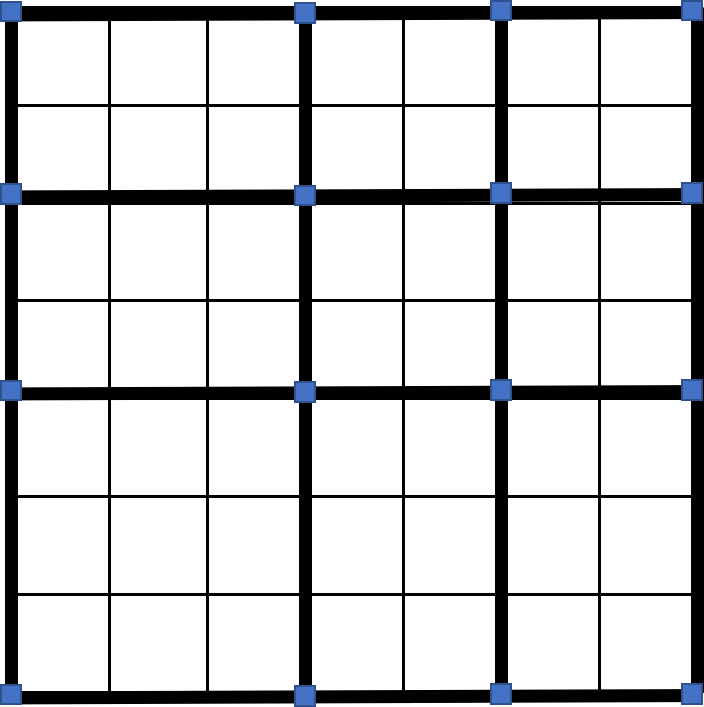
\includegraphics[width=6cm]{figs/grosso.png}
\caption{Exemplo de grid fino 7x7 e um grid grosso 3x3. O elemento inferior esquerdo é composto por 9 elementos do grid fino enquanto o elemento superior direito é composto com 4 elementos do grid fino.}
\end{figure}


Na seção\ref{ch:discretizacao} foi apresentada a discretização através de elementos finitos para o problema de elasticidade linear através do método dos elementos finitos. A notação utilizada é baseada na utilizada em \cite{mbuck}. Assim, como no método dos elementos finitos em que se deseja aproximar a função em um espaço $V^h$ formado por funções de base chapéu no domínio $\Omega$ do problema, a ideia agora é encontrar a solução do problema em um espaço grosso $V^{H}$, tal que $V^{H} \subset V^h$. 



Para definir melhor esse espaço $V^{H}$ precisamos definir as suas funções de base geradoras dele assim como foram definidas para $V^h$.  Novamente, para distinguir o nó pertencente ao grid grosso dos seus graus de liberdade o seguinte conjunto com graus de liberdade é criado.


\begin{equation}
    D^H = \{ p^{(m)} \in D^h : x^p \in \Sigma_H, m=1,2\}
\end{equation}
Onde, \(\Sigma_H\) representa o conjunto de nós do grid grosso e \(D^h\) os graus de liberdade do grid fino. Além disso, deve-se considerar o conjunto

\begin{equation}
    S_p = \{T \in \tau_H : x^p \in T\}
\end{equation}que representa os elementos grossos relacionados ao nó grosso $x^p $. A nova solução encontrada no grid grosso será uma combinação linear das funções de base $\phi_{j{(k)}}^H : \mathbb{R}^2 \mapsto \mathbb{R}^2 $  .
\begin{equation}
u^H = 
\begin{bmatrix}
u^H_x
\\ 
u^H_y
\end{bmatrix}
= \sum_{j=1}^{n_P} u_{j^{(k)}} \phi^H_{j^{(k)}}
\end{equation}

Onde essas funções de de base do grid grosso são calculadas resolvendo problemas locais de modo que elas possuam informação do operador original e $\phi^H_{p^{(k)}}$  possui suporte em $S_p$.  Um representação do $S_6$ é apresentada em figura \ref{fig:s6}

\begin{figure}[!htbp]
\label{fig:s6}
\centering
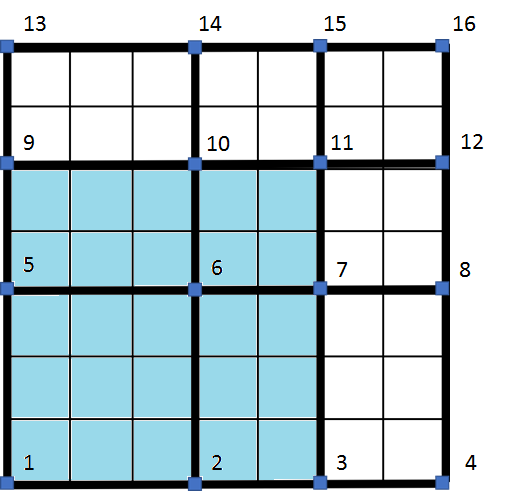
\includegraphics[width=6cm]{figs/S6.png	}
\caption{Exemplo de conjunto $S_6$ que define o suporte das funções  $\phi^H_{6^{(1)}}$ e  $\phi^H_{6^{(2)}}$ no caso 2D}
\end{figure}


Como apresentado em \cite{casteletto}, os problema locais para o cálculo de cada função de base é  composto pelas equações apresentadas em \ref{eq:problemalocal}. 

\begin{equation} \label{eq:problemalocal}
\left\{\begin{matrix}
\nabla \cdotp (C:\nabla ^ S \phi^H_{j^{(k)}}) = \mathbf{0}, \text{   em  } T
\\ 
\nabla_{||} \cdotp (C:\nabla_{||} ^ S \phi^H_{j^{(k)}}) = \mathbf{0}, \text{  em   } \partial T
\\ 
\phi^H_{j^{(k)}} = \delta_{jp} e_k, \text{    em   } x^p \in \Sigma ^ H
\end{matrix}\right.
\end{equation} onde $e_k$ representa um vetor com o valor igual a 1 na posição k, ou seja, no caso de duas dimensões $e_0 = [1, 0]^T$ e $e_1  = [0, 1]^T$ e $T \in S_j$ . No caso de 2 dimensões com elementos quadriláteros, cada função de base será calculada através da solução de 4 problemas locais pois cada nó pertence a quatro elementos diferentes. 

Além de satisfazer as equações \ref{eq:problemalocal}, as funções de base do grid grosso são também selecionadas de forma ser uma combinação linear das funções de base do grid fino como mostra a a equação \ref{eq:baseGrossoXbaseFino}


\begin{equation} \label{eq:baseGrossoXbaseFino}
    \phi^H_{i^{(k)}} = \sum_{j} p_{ij} \phi^h_{j}
\end{equation}

Dessa forma, é necessário encontrar os coeficientes $p_{ij}$ de forma a definir exatamente as funções de base de $V^H$. E, juntando \ref{eq:problemalocal} com \ref{eq:baseGrossoXbaseFino}, pode-se resolver encontrar esses valores utilizando o método dos elementos finitos.


\subsection{Resolução dos Problemas Locais}

Para a solução dos problemas apresentados pelas equações \ref{eq:problemalocal} com \ref{eq:baseGrossoXbaseFino}, é possível adotando o seguinte procedimento, primeiramente se resolve o problema em $\partial T$ e depois se resolve o problema para o interior $T$. É importante perceber que o problema em $\partial T$ é um problema 1D quando o problema original é apresentado em 2D. 


Portanto, para o nó $x^6$ do grid grosso está relacionado com duas funções de base do grid grosso $\phi^H_{6^{(1)}}$ e  $\phi^H_{6^{(2)}}$  com suporte em $S_6$. Para cada uma das funções é necessário resolver quatro problemas, um para cada um dos elementos $T_1$, $T_2$, $T_4$ e $T_5$. Tomando o problema do elemento $T_4$ como base. Como citado inicialmente se resolve o problema em $\partial T_4$ utilizando a segunda e terceira equação de \ref{eq:problemalocal}. De acordo com a terceira equação, os valores de estão definidos nos nós $x^5$, $x^6$, $x^9$ e $x^{10}$. No caso,


\begin{equation}
    \left\{\begin{matrix} \label{eq:phi6_values}
\phi^H_{6^{(1)}} (x⁵) = [0, 0]^T && \phi^H_{6^{(2)}} (x⁵) = [0, 0]^T
\\ 
\phi^H_{6^{(1)}} (x^6) = [1, 0]^T && \phi^H_{6^{(2)}} (x^6) = [0, 1]^T
\\ 
\phi^H_{6^{(1)}}(x^9) = [0, 0]^T && \phi^H_{6^{(2)}} (x^9 ) = [0, 0]^T
\\
\phi^H_{6^{(1)}}(x^{10}) = [0, 0]^T && \phi^H_{6^{(2)}} (x^{10}) = [0, 0]^T
\end{matrix}\right.
\end{equation}

É importante perceber que os valores de $\phi^H_{6^{(1)}}$ e $\phi^H_{6^{(2)}}$ são $ [0, 0] ^T  $ para as fronteiras relacionadas ao segmentos entre os pontos $x^9$ e $x^{10}$ e $x^5$ e $x^9$ . A figura \ref{fig:phi6_values} mostra em vermelho as regiões de $\partial T_4 $ onde as funções são $\mathbf{0}$  e em verde as regiões onde é necessário resolver a EDP \ref{eq:problemalocal} juntamente com a condição de contorno de \ref{eq:phi6_values}.

 


\begin{figure}[!htbp]
\label{fig:phi6_values}
\centering
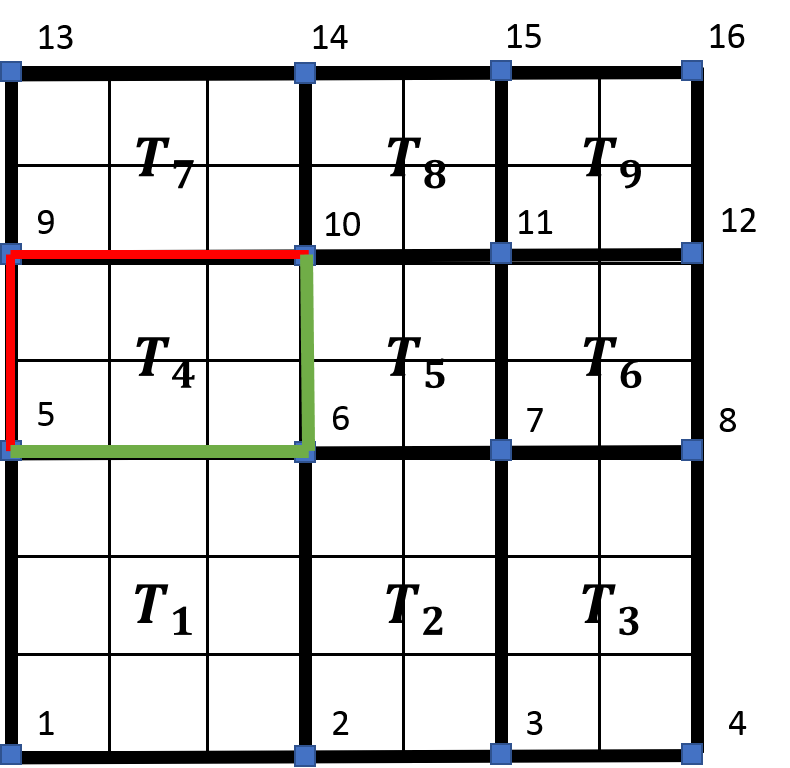
\includegraphics[width=6cm]{figs/phi6_values.png}
\caption{Em vermelho é apresentado onde os valores de \phi^H_{6^{(1)}} e \phi^H_{6^{(2)}} tem valor $\mathbf{0}$ e em verde onde problemas 1D tem que ser resolvidos para encontrar os valores das funções;}
\end{figure}

De acordo com \cite{casteletto}, através de uma mudança de variável dos eixos $x$ e $y$ para eixos $\hat{x}$ e $\hat{y}$ que representam respectivamente a direção  paralela a fronteira e a direção normal a fronteira pode se transformar a \ref{eq:problemalocal} em \ref{eq:mudancadevariavel}.  A figura 


\begin{equation} 
    \left\{\begin{matrix} \label{eq:mudancadevariavel}
\frac{\partial}{\partial \hat{x}}(K_v \frac{\partial}{\partial \hat{x}})
\\ 
\frac{\partial}{\partial \hat{y}}(G \frac{\partial}{\partial \hat{y}})
\end{matrix}\right.
\end{equation}

\begin{figure}[!htbp]
\label{fig:mudancadevariavel}
\centering
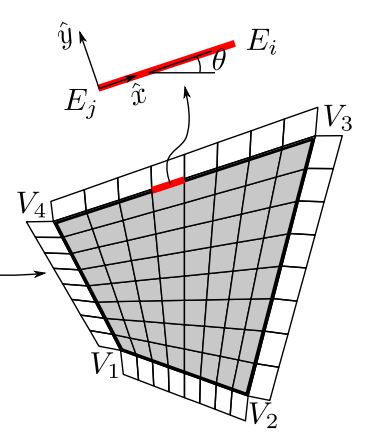
\includegraphics[width=6cm]{figs/mudancadevariavel.png}
\caption{Em vermelho é apresentado onde os valores de \phi^H_{6^{(1)}} e \phi^H_{6^{(2)}} tem valor $\mathbf{0}$ e em verde onde problemas 1D tem que ser resolvidos para encontrar os valores das funções;}
\end{figure}

\section{Resultados}


\section{Conclusão}
``I always thought something was fundamentally wrong with the universe'' \citep{adams1995hitchhiker}

\bibliographystyle{plain}
\bibliography{references}
\end{document}
